
\section{shallow ice sheets}

\begin{frame}{slow, non-Newtonian, shallow, and sliding}

\begin{itemize}
\item ice sheets have four outstanding properties \emph{as fluids}:
  \begin{enumerate}
  \item slow
  \item non-Newtonian
  \item shallow (at big scale)
  \item<1> contact slip (some places, sometimes)
  \end{enumerate}

\bigskip
\item<2> our first model captures the first three properties
\end{itemize}
\end{frame}


\begin{frame}{regarding ``shallow''}

\begin{itemize}
\item below in \alert{red} is a no-vertical-exaggeration cross section of Greenland at $71^\circ$
\small
\item green and blue: standard vertically-exaggerated cross section

\medskip
\begin{center}
  \includegraphics[width=0.6\textwidth]{green_transect}
\end{center}

\medskip
\footnotesize
\item \emph{note}: you can scale Stokes equation using smallness of $\eps = [H]/[L]$, where $[H]$ is a typical thickness of an ice sheet and $[L]$ is a typical horizontal dimension, \dots (see Chapter 18 of Fowler, 1997)\nocite{Fowler}
\end{itemize}
\end{frame}


\subsection{shallow ice approx (SIA)}

\begin{frame}{flow model I: non-sliding, isothermal shallow ice approximation (= SIA)}

a model which applies to
\begin{itemize}
\item small depth-to-width ratio (``shallow'') grounded ice sheets
\item on not-too-rough bed topography,
\item whose flow is not dominated by sliding and/or liquid water at the base or margin
\end{itemize}

\begin{center}
  \includegraphics[width=0.65\textwidth]{polaris}

\tiny ``Polaris Glacier,'' northwest Greenland, photo 122, Post \& LaChapelle (2000)\nocite{PostLaChapelle}
\end{center}

\end{frame}


\begin{frame}{SIA velocity equation}

\begin{itemize}
\item instead of an $\epsilon = [H]/[L]$ argument, here we take the simple slogan:

\begin{center}
\alert{the SIA uses the formulas from slab-on-a-slope}
\end{center}
\item shear stress approximation:
	$$(\tau_{13},\tau_{23}) = - \rho g (h-z) \nabla h$$
\item let $\mathbf{U} = (u,v)$ be the horizontal velocity
\item we further approximate
\begin{align*}
\mathbf{U}_z &= 2 A |(\tau_{13},\tau_{23})|^{n-1} (\tau_{13},\tau_{23}) \\
     &= - 2 A (\rho g)^n (h-z)^n |\nabla h|^{n-1} \nabla h
\end{align*}
\item by integrating vertically, in the non-sliding case,
    $$\mathbf{U} = - \frac{2 A (\rho g)^n}{n+1} \left[H^{n+1} - (h-z)^{n+1}\right] |\nabla h|^{n-1} \nabla h$$
\end{itemize}
\end{frame}


\begin{frame}{SIA thickness equation}

\begin{itemize}
\item but mass continuity remains:
  $$H_t = M - \Div \left(\overline{\mathbf{U}} H\right)$$
\item from velocity formula for $\mathbf{U}$ on last slide, combine to get the non-sliding, isothermal shallow ice approximation:
\begin{equation}
H_t = M + \Div \left(\Gamma H^{n+2} |\grad h|^{n-1} \grad h \right) \notag
\end{equation}

  \begin{itemize}
  \item[$\circ$] where $H$ is ice thickness, $h$ is ice surface elevation, $b$ is bed elevation ($h=H+b$)
  \item[$\circ$] $M$ combines surface and basal mass (im)balance:

     accumulation if $M>0$, ablation if $M<0$
  \item[$\circ$] $n$ is the exponent in the Glen flow law
  \item[$\circ$] $\Gamma = 2 A (\rho g)^n / (n+2)$ is a positive constant
  \end{itemize}
\end{itemize}
\end{frame}


\begin{frame}{the SIA model}

\begin{itemize}
\item the SIA equation from last slide:
\begin{empheq}[box=\fbox]{equation}
H_t = M + \Div \left(\Gamma H^{n+2} |\grad h|^{n-1} \grad h \right) \label{sia}
\end{empheq}
\item equation (1) describes how ice thickness varies in time and space, as a function of climate $M$ and bed elevation $b$
\item numerically solve (1) and you've got a usable model for \dots \emph{the Barnes ice cap} (Mahaffy, 1976; model-observation fit below)\nocite{Mahaffy}
\end{itemize}

\begin{columns}
\begin{column}{0.7\textwidth}
\small
\noindent good questions:
\begin{enumerate}
\item where does equation (1) come from?\only<2>{\qquad \checkmark}
\item \only<1>{how to solve it numerically?} \only<2>{\alert{how to solve it numerically?}}
\item \only<1>{how to \emph{think} about it?} \only<2>{\alert{how to \emph{think} about it?}}
\end{enumerate}  
\end{column}
\begin{column}{0.3\textwidth}
\vspace{-3mm}
\includegraphics[width=1.0\textwidth]{mahaffy-profiles}
\end{column}
\end{columns}
\end{frame}


\subsection{analogy w heat equation}

\begin{frame}{heat equation (as analogy for SIA)}

\begin{columns}
\begin{column}{0.75\textwidth}
\begin{itemize}
\item recall Newton's law of cooling
	$$\frac{dT}{dt} = -K (T-T_{\text{ambient}})$$
where
  \begin{itemize}
  \item[$\circ$] where $T$ is object temperature and
  \item[$\circ$] $K$ relates to material and geometry of object
  \end{itemize}

\bigskip
\item e.g.~hot cup of coffee in lecture room

\bigskip
\item solution:
  $$\text{exponential decay of $T(t)$ to $T_{\text{ambient}}$}$$
\end{itemize}
\end{column}

\begin{column}{0.25\textwidth}
\vspace{1.0in}

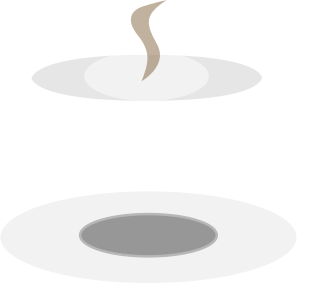
\includegraphics[width=0.9\textwidth]{coffee}
\end{column}
\end{columns}
\end{frame}


\begin{frame}{heat equation (as analogy for SIA) \qquad 2}

\begin{columns}
\begin{column}{0.7\textwidth}
\begin{itemize}
\item Newton's law for segments of a rod:
\begin{align*}
\frac{dT_j}{dt} &= -K \left(T_j - \frac{1}{2} (T_{j-1} + T_{j+1}) \right) \\
	&= \frac{K}{2} \left(T_{j-1} - 2 T_j + T_{j+1}\right) 
\end{align*}
\item \dots because average of neighbor's temperatures \emph{is} ambient 
\item has this limit as segments shrink:
	$$T_t = D T_{xx}$$
where
  \begin{itemize}
  \item[$\circ$] $D$ is ``diffusivity''
  \item[$\circ$] $D$ includes material properties: conductivity, density, heat capacity
  \end{itemize}

\medskip
\small
\item see also: ``finite difference approximations''
\end{itemize}
\end{column}

\begin{column}{0.3\textwidth}
\vspace{5mm}

\hspace{-10mm}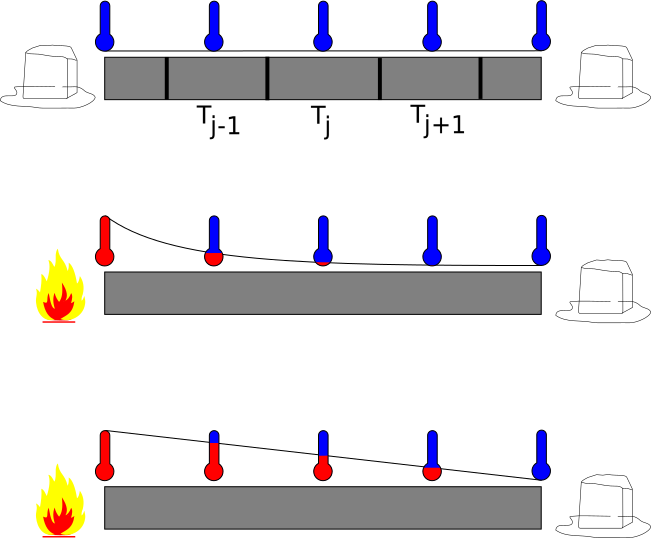
\includegraphics[width=1.3\textwidth]{heatconduction}
\end{column}
\end{columns}
\end{frame}


\begin{frame}{2D heat equation}

\begin{columns}
\begin{column}{0.6\textwidth}
\begin{itemize}
\item $T(t,x,y)$ is temperature in object at position $x,y$ and time $t$
\item Fourier rewrote Newton's law as a rule for heat flux: $\mathbf{q} = - k \grad T$
\item also: $\rho$ is density, $c$ is specific heat, $k$ is conductivity, $f$ is heat source
\item by conservation of energy:
	$$\rho c T_t = f + \Div (k \grad T)$$
\item define $D = k/(\rho c)$ and $F = f/(\rho c)$
\item get heat equation:
\begin{equation}
T_t = F + \Div (D\, \grad T) \label{heat}
\end{equation}
\end{itemize}
\end{column}

\begin{column}{0.4\textwidth}
\mode<presentation>{
\animategraphics[autoplay,loop,height=2.5cm]{4}{../anim/heatmelt}{0}{16}
}
\end{column}
\end{columns}
\end{frame}


\begin{frame}{analogy: SIA versus 2D heat equation}

\begin{itemize}
\item side-by-side comparison of (1) and (2):
\smallskip

\hspace{-7mm}
\begin{tabular}{cc}
\scriptsize SIA:\, $H(t,x,y)$ is ice thickness & \scriptsize heat: $T(t,x,y)$ is temperature \normalsize \\
	\boxed{H_t = M + \Div \left({\color{red}\Gamma H^{n+2} |\grad h|^{n-1}}\, \grad h \right)}  &  \boxed{T_t = F + \Div (D\, \grad T)}
\end{tabular}

\medskip
\item we identify the diffusivity in the SIA:
	$$D = {\color{red}\Gamma H^{n+2} |\grad h|^{n-1}}$$
\item \emph{non-sliding shallow ice flow \alert{diffuses} the ice sheet}
\item some issues with this analogy:
  \begin{itemize}
  \item[$\circ$]  $H$ and $h$ are different \dots but at least $H=h+b$
  \item[$\circ$]  $D$ depends on $H$, the solution
  \item[$\circ$]  $D\to 0$ at margin, where $H\to 0$
  \item[$\circ$]  $D\to 0$ at divides/domes, where $|\grad h|\to 0$
  \end{itemize}
\medskip
\item<2> \emph{we are finally ready for numerics!} 
\end{itemize}

\end{frame}


\subsection{finite difference numerics}

\begin{frame}{numerics for heat equation: basic ideas of finite differences}

\begin{itemize}
\item numerical schemes for heat equation are good start for SIA
\item for differentiable $f(x)$ and any $h$, \emph{Taylor's theorem} says
	$$f(x+h) = f(x) + f'(x) h + \frac{1}{2} f''(x) h^2 + \frac{1}{3!} f'''(x) h^3 + \dots$$
\normalsize
\item you can replace ``$h$'' by multiples of $\Delta x$, e.g.:
\small
\begin{align*}
f(x-\Delta x) &= f(x) - f'(x) \Delta x + \frac{1}{2} f''(x) \Delta x^2 - \frac{1}{3!} f'''(x) \Delta x^3 + \dots \\
f(x+2\Delta x) &= f(x) + 2 f'(x) \Delta x + 2 f''(x) \Delta x^2 + \frac{4}{3} f'''(x) \Delta x^3 + \dots
\end{align*}
\normalsize
\item \emph{combine expressions like these to give approximations of derivatives, from values on a grid}
\end{itemize}
\end{frame}


\begin{frame}{finite differences for partial derivatives}

\begin{itemize}
\item we want partial derivative expressions, for example with any function $u=u(t,x)$:
\small
\begin{align*}
u_t(t,x) &= \frac{u(t+\Delta t,x) - u(t,x)}{\Delta t} + O(\Delta t), \\
u_t(t,x) &= \frac{u(t+\Delta t,x) - u(t-\Delta t,x)}{2\Delta t} + O(\Delta t^2), \\
u_x(t,x) &= \frac{u(t,x+\Delta x) - u(t,x-\Delta x)}{2\Delta x} + O(\Delta x^2), \\
u_{xx}(t,x) &= \frac{u(t,x+\Delta x) - 2 u(t,x) + u(t,x-\Delta x)}{\Delta x^2} + O(\Delta x^2)
\end{align*}
\normalsize
and so on
\item sometimes we want a derivative in-between grid points:
\small
	$$u_x(t,x+(\Delta x/2)) = \frac{u(t,x+\Delta x) - u(t,x)}{\Delta x} + O(\Delta x^2)$$
\normalsize
\item ``$+O(h^2)$'' is better than ``$+O(h)$'' if $h$ is a small number
\end{itemize}
\end{frame}


\begin{frame}{explicit scheme for heat equation}

\begin{itemize}
\item consider 1D heat equation $T_t = D T_{xx}$
\item an \emph{explicit} scheme comes from:
\small
	$$\frac{T(t+\Delta t,x) - T(t,x)}{\Delta t} \approx D\,\frac{T(t,x+\Delta x) - 2 T(t,x) + T(t,x-\Delta x)}{\Delta x^2}$$
\normalsize
\item more notation:
  \begin{itemize}
  \item[$\circ$] $(t_n,x_j)$ denotes a point in a time-space grid
  \item[$\circ$] $T_j^n \approx T(t_n,x_j)$
  \item[$\circ$] $\nu = D \Delta t / (\Delta x)^2$
  \end{itemize}
\end{itemize}

\begin{columns}
\begin{column}{0.6\textwidth}
\begin{itemize}
\item then scheme is
	$$T_j^{n+1} = \nu T_{j+1}^n + (1 - 2 \nu) T_j^n + \nu T_{j-1}^n$$
\item stencil \large $\to$ \normalsize
\end{itemize}
\end{column}
\begin{column}{0.4\textwidth}
\hspace{5mm}\includegraphics[width=0.8\textwidth]{expstencil}
\end{column}
\end{columns}
\end{frame}


\begin{frame}{explicit scheme in two space dimensions}

\begin{itemize}
\item a heat equation in 2D: \quad $T_t = D(T_{xx} + T_{yy})$
\item we write $T_{jk}^n \approx T(t_n,x_j,y_k)$
\item the 2D explicit scheme is
\small
	$$\frac{T_{jk}^{n+1} - T_{jk}^n}{\Delta t} = D\,\left(\frac{T_{j+1,k}^n - 2 T_{jk}^n + T_{j-1,k}^n}{\Delta x^2} + \frac{T_{j,k+1}^n - 2 T_{jk}^n + T_{j,k-1}^n}{\Delta y^2}\right)$$
\normalsize
\item space-only stencil below
\end{itemize}

\bigskip
\begin{center}
\includegraphics[width=0.4\textwidth]{exp2dstencil}
\end{center}
\end{frame}


\begin{frame}{implementation}

\minput{heat}

\small
\begin{itemize}
\item solves $T_t = D(T_{xx} + T_{yy})$ on square $-1 < x < 1$, $-1 < y < 1$
\item example uses gaussian initial condition $T(0,x,y) = e^{-30 r^2}$
\item uses ``colon notation'' to remove loops
\item \texttt{>>  heat(1.0,30,30,0.001,20)}

approximates $T$ on $30\times 30$ spatial grid, with $D=1$; take $N=20$ steps of $\Delta t = 0.001$ to final time $t = 0.02$
\end{itemize}
\end{frame}


\begin{frame}{the look of success}

\begin{columns}
\begin{column}{0.5\textwidth}
initial condition $T(0,x,y)$

\bigskip
\begin{center}
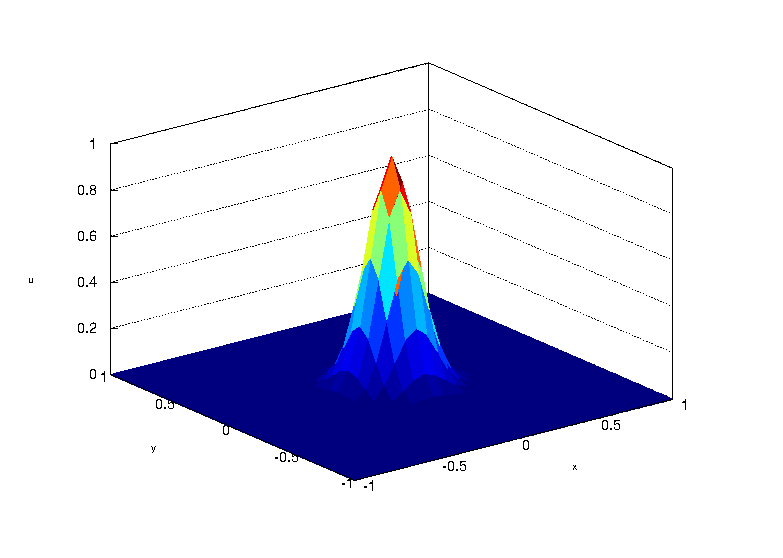
\includegraphics[width=1.0\textwidth]{initialheat}
\end{center}
\end{column}
\begin{column}{0.5\textwidth}
approximate solution $T(t,x,y)$ at $t=0.02$

\bigskip
\begin{center}
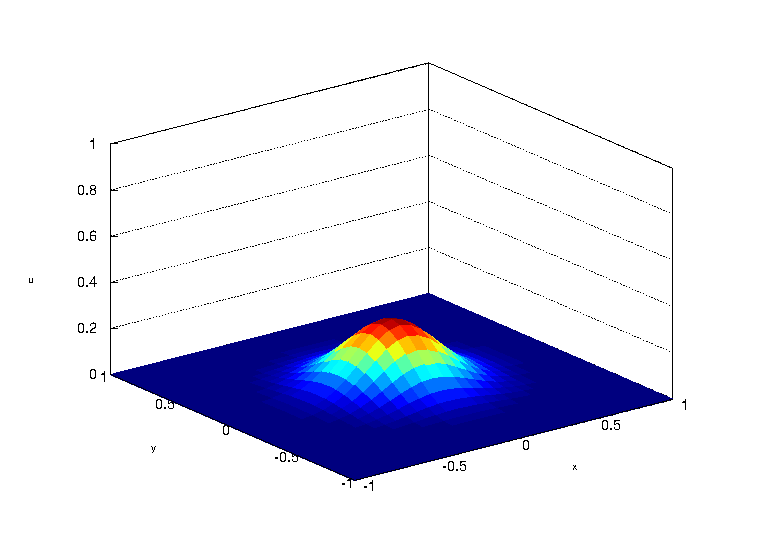
\includegraphics[width=1.0\textwidth]{finalheat}
\end{center}
\end{column}
\end{columns}
\end{frame}


\begin{frame}{the look of instability}

\begin{itemize}
\item both figures are from solving $T_t = D(T_{xx} + T_{yy})$ on the \emph{same} space grid and the \emph{same} final time
\item \dots but with slightly different time steps
\end{itemize}

\medskip
\begin{columns}
\begin{column}{0.5\textwidth}
\begin{center}
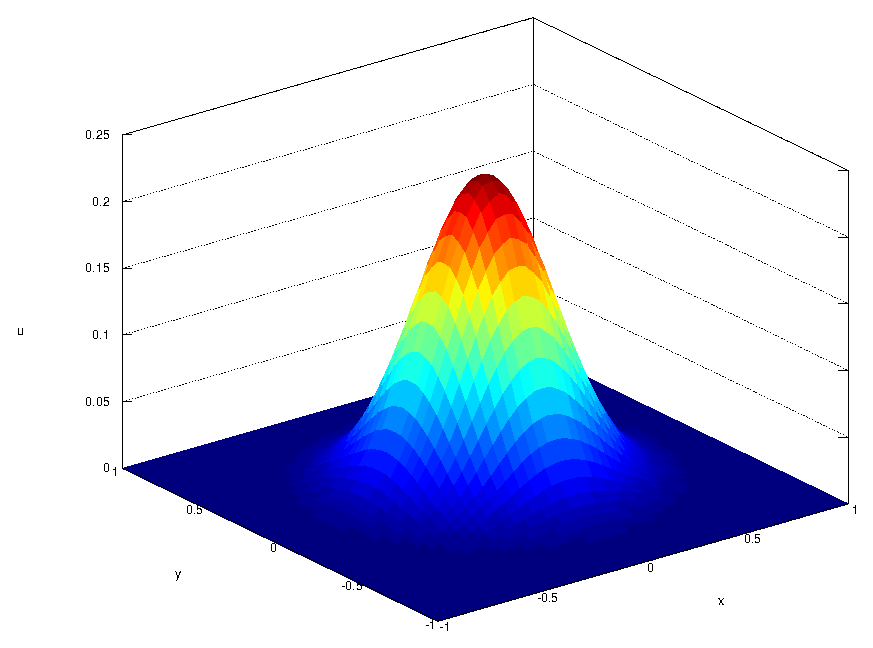
\includegraphics[width=1.0\textwidth]{stability}
% >> heat(1,80,80,0.0001,200);
% $D=1,J=K=80,\Delta t = 0.0001,N=200$
% so $t_f=0.02,\Delta x = \Delta y = 0.025$ so
\medskip
\small
  $$\Delta t=0.0001 \, \text{ and } \, \frac{D\Delta t}{\Delta x^2}= 0.16$$
\end{center}
\end{column}
\begin{column}{0.5\textwidth}
\begin{center}
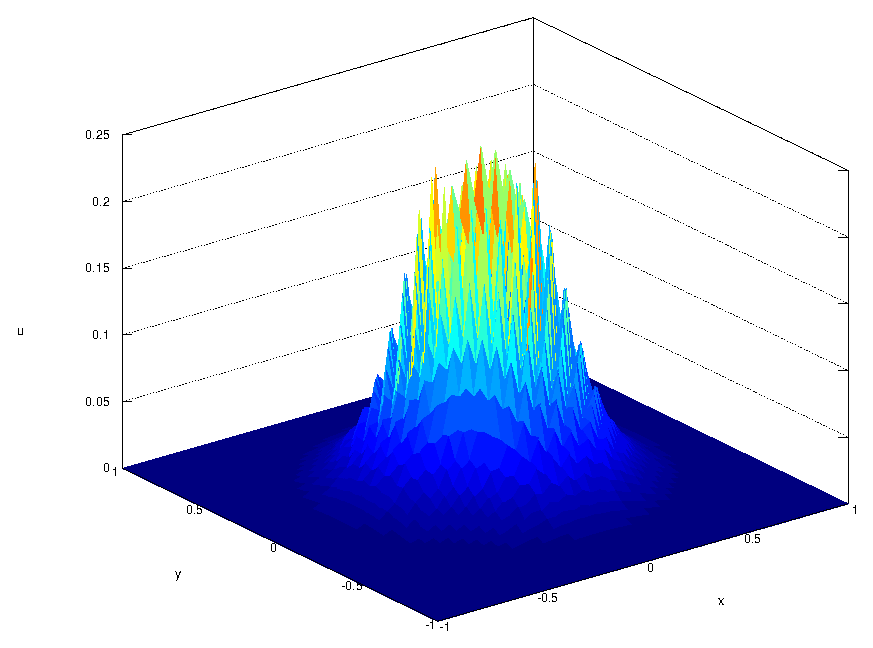
\includegraphics[width=1.0\textwidth]{instability}
% >> heat(1,80,80,0.0002,100);
% $D=1,J=K=80,\Delta t = 0.0002,N=100$
% so $t_f=0.02,\Delta x = \Delta y = 0.025$ so
\small
\smallskip
  $$\Delta t=0.0002 \, \text{ and } \, \frac{D\Delta t}{\Delta x^2}= 0.32$$
\end{center}
\end{column}
\end{columns}
\end{frame}


\begin{frame}{understand and avoid the instability}

\begin{itemize}
\item recall 1D explicit scheme had the form 
	$$T_j^{n+1} = \nu T_{j+1}^n + (1 - 2 \nu) T_j^n + \nu T_{j-1}^n$$
\item thus the new value $T_j^{n+1}$ is an \emph{average} of the old values, \emph{if the middle coefficient is positive}:
	$$1 - 2 \nu \ge 0 \quad \iff \quad  \frac{D\Delta t}{\Delta x^2} \le \frac{1}{2} \quad \iff \quad \Delta t \le \frac{\Delta x^2}{2 D}$$
\item averaging is stable because averaged wiggles are smaller than the original wiggles
\item \emph{the result was unstable because the time step was too big}

\item in 2D case with $\Delta x = \Delta y$ the condition is
	$$\frac{D\Delta t}{\Delta x^2} \le \frac{1}{4}$$
\vspace{-3mm}
\item this condition is a sufficient \alert{stability criterion}
\end{itemize}
\end{frame}


\begin{frame}{adaptive implementation: guaranteed stability}

\minput{heatadapt}

\begin{itemize}
\item same as \texttt{heat.m} except

\begin{center}
\alert{time step computed from stability criterion}
\end{center}
\end{itemize}\end{frame}


\begin{frame}{alternative instability fix: implicitness}

\begin{itemize}
\item \alert{implicit} methods can be stable for \emph{any} positive time step $\Delta t$
\end{itemize}

\begin{columns}
\begin{column}{0.7\textwidth}
\begin{itemize}
\item an implicit scheme is \emph{Crank-Nicolson} $\longrightarrow$
\item Crank-Nicolson has smaller error too
\end{itemize}
\normalsize
\end{column}
\begin{column}{0.3\textwidth}
\includegraphics[width=1.2\textwidth]{cnstencil}
\end{column}
\end{columns}

\begin{itemize}
\item \emph{but} you have to solve a linear (for heat equation) system of equations to take each time step
  \small
  \begin{itemize}
  \item[$\circ$] becomes a \emph{nonlinear} system of equations at each time step for ice flow
  \item[$\circ$] implementation of nonlinear solver is an ``opportunity cost''
  \item[$\circ$] \dots never address the other processes you really care about?
  \end{itemize}

\bigskip
\item Donald Knuth has advice for ice sheet modelers: \begin{quote}
\emph{We should forget about small efficiencies \dots: premature optimization is the root of all evil}.
\end{quote}
\end{itemize}
\end{frame}


\begin{frame}{variable diffusivity and staggered grid}

\begin{itemize}
  \item recall the analogy: \qquad (SIA) $\leftrightarrow$ (heat eqn)
  \item the SIA has a diffusivity which varies in space, so consider a more general heat equation:
  		$$T_t = F + \Div \left(D(x,y) \grad T\right)$$
  \item the explicit method is conditionally stable with the same time step restriction if we evaluate diffusivity $D(x,y)$ at \alert{staggered} grid points:
  \scriptsize\vspace{-4mm}
\begin{align*}
\Div \left(D(x,y) \grad T\right) &\approx \frac{D_{j+1/2,k}(T_{j+1,k} - T_{j,k}) - D_{j-1/2,k}(T_{j,k} - T_{j-1,k})}{\Delta x^2} \\
	&\qquad + \frac{D_{j,k+1/2}(T_{j,k+1} - T_{j,k}) - D_{j,k-1/2}(T_{j,k} - T_{j,k-1})}{\Delta y^2}
\end{align*}
\end{itemize}

\small
\begin{columns}
\begin{column}{0.5\textwidth}
in stencil at right:
\begin{itemize}
\item[] diamonds: $T$
\item[] triangles: $D$
\end{itemize}
\end{column}
\begin{column}{0.5\textwidth}
\hfill\includegraphics[width=0.6\textwidth]{diffstencil}
\end{column}
\end{columns}
\end{frame}


\begin{frame}
  \frametitle{general diffusion equation code}

\minputtiny{diffusion}

\small
\begin{itemize}
\item solves abstract diffusion equation $T_t = \Div \left(D(x,y)\, \grad (T+b)\right)$
\item user supplies diffusivity on staggered grid
\end{itemize}
\end{frame}


\subsection{solutions}

\begin{frame}{verification of numerical ice flow codes}
\begin{itemize}
\item STOP! \quad the code on the last slide is complicated!

\bigskip
\item<2-> how do we make sure an \emph{implemented} numerical scheme is correct?
  \begin{itemize}
  \item<3->[\emph{technique} 1] don't make any mistakes
  \item<4->[\emph{technique} 2] compare your model with others, and hope that the outliers are the ones with errors \only<4>{$=$ \alert{intercomparison}}
  \item<5>[\emph{technique} 3] compare your model to an exact solution, and actually measure the numerical error \only<5>{$=$ \alert{verification}}
  \end{itemize}
\end{itemize}
\end{frame}


\begin{frame}{verification of numerical ice flow codes \quad 2}
\begin{itemize}
\item<1-> yeah, BUT where do you get exact solutions for ice flow models!?
  \begin{itemize}
  \item[$\circ$] textbook with several SIA solutions: van der Veen (2013)
  \item[$\circ$] similarity solutions to SIA (Halfar 1983; Bueler et al 2005)
  \item[$\circ$] flowline SSA solutions (B\"o\dh varsson, 1955; van der Veen, 1983; Bueler, 2014)
  \item[$\circ$] cross-flow SSA solution (Schoof, 2006)
  \item[$\circ$] flowline Stokes solutions for constant viscosity (Balise and Raymond 1985)
  \end{itemize}

\item<1-> if desperate, ``manufacture'' an exact solution
  \begin{itemize}
  \item[$\circ$] to thermo-coupled SIA (Bueler et al 2007)
  \item[$\circ$] to flowline Blatter (Glowinski and Rappaz 2003)
  \item[$\circ$] to the Glen-law Stokes equations (Sargent and Fastook 2010; Jouvet and Rappaz 2011; Leng et al 2014)
  \end{itemize}

\smallskip
\item<2> Ed says:
\begin{center}
\emph{not having an exact solution is a sign that you don't understand the continuum model well enough}
\end{center}
\end{itemize}
\end{frame}


\begin{frame}{e.g.~exact solution of heat equation}

\begin{itemize}
\item recall 1D heat equation with constant diffusivity:
	$$T_t = D T_{xx}$$
\item many exact solutions to the heat equation are known

\bigskip
\item here we find the ``Green's function''
  \begin{itemize}
  \item[$\circ$] a.k.a.~``fundamental solution'' or ``heat kernel''
  \item[$\circ$] starts at time $t=0$ with a ``delta function'' of heat at the origin $x=0$ and then it spreads out over time
  \item[$\circ$] we find it by a method which generalizes to the SIA
  \end{itemize}
\end{itemize}
\end{frame}


\begin{frame}{Green's function of heat equation}

\begin{itemize}
\item the solution is ``self-similar'' over time
\item as time increases it changes shape by
  \begin{itemize}
  \item[$\circ$] shrinking the output (vertical) axis and
  \item[$\circ$] lengthening the input (horizontal) axis
  \end{itemize}
\item \dots\, but otherwise it always has the same shape
  \begin{itemize}
  \item[$\circ$] by conservation of energy, integral over $x$ independent of time
  \end{itemize}
\end{itemize}

\begin{center}
\includegraphics[width=0.5\textwidth]{heatscaling}

\emph{increasing time} \Large $\to$
\end{center}
\end{frame}


\begin{frame}{similarity solutions}

\begin{itemize}
\item Green's function of 1D heat equation ($T_t = D T_{xx}$) is
	$$T(t,x) = C\, t^{-1/2} e^{-x^2/(4Dt)}$$
\item ``similarity'' variable is $s = t^{-1/2} x$
  \begin{itemize}
  \item[$\circ$] \emph{historical note}:  in 1905 Einstein saw that the average distance traveled by particles in thermal motion scales like $\sqrt{t}$, so $s = t^{-1/2} x$ is an invariant

  \vspace{-2mm}
  \hfill\includegraphics[width=0.25\textwidth]{brownian}
  \end{itemize}
\item similarity solution as scaling:
	$$s \stackrel{\text{\emph{input scaling}}}{\phantom{\Big|}=\phantom{\Big|}} t^{-1/2} x, \qquad T(t,x) \stackrel{\text{\emph{output scaling}}}{\phantom{\Big|}=\phantom{\Big|}} t^{-1/2} \phi(s)$$
where
    $$\phi(s) = C e^{-s^2/(4D)}$$
\end{itemize}

\end{frame}


\subsection{solving the SIA}

\begin{frame}{similarity solution to SIA}

\begin{itemize}
\item jump forward to 1981
\item P.~Halfar found the similarity solution of the SIA in the case of flat bed and no surface mass balance \nocite{Halfar81,Halfar83}
\item Halfar's 2D solution for Glen flow law with $n=3$ has scalings
   $$H(t,r)={\color{red} t^{-1/9}} \phi(s), \qquad s = {\color{blue} t^{-1/18}} r$$
  \begin{center}
  \includegraphics[width=0.4\textwidth]{halfarscalings}
  \end{center}
\item \dots so the diffusion of ice really slows down as time goes on
\end{itemize}
\end{frame}


\begin{frame}{Halfar solution to the SIA: the movie}

\animategraphics[autoplay,loop,height=7.0cm]{4}{../anim/halfar}{0}{26}

\par
\scriptsize 
frames from $t=4$ months to $t = 10^6$ years, equal spaced in \emph{exponential} time
\end{frame}


\begin{frame}{Halfar solution to the SIA: the formula}

\begin{itemize}
\item for $n=3$:
  $$H(t,r) = H_0 \left(\frac{t_0}{t}\right)^{1/9} \left[1 - \left(\left(\frac{t_0}{t}\right)^{1/18} \frac{r}{R_0}\right)^{4/3}\right]^{3/7}$$
where $H_0$, $R_0$ are center height and ice cap radius at $t=t_0$
\item the ``characteristic time'' is
  $$t_0 = \frac{1}{18 \Gamma} \left(\frac{7}{4}\right)^3 \frac{R_0^4}{H_0^{7}}$$
(e.g.~choose $H_0$ and $R_0$; this determines $t_0$)
\item it is an easy formula to use for verification!
\item code \texttt{verifysia.m} (not shown) uses it
\end{itemize}
\end{frame}


\begin{comment}
\begin{frame}{on ``degenerate'' diffusivity}

\begin{itemize}
\item recall that the SIA is
\small
	$$H_t = M + \Div \left(D\, \grad h \right) \quad \text{where} \quad D = \Gamma H^{n+2} |\grad h|^{n-1}$$
\normalsize
\item thus the diffusivity ``degenerates'', $D \to 0$, when either $H\to 0$ or $\grad h \to 0$
\item summary:
\small
\begin{tabular}{l|c|c}
 & why $D\to 0$ & so what? \\ \hline
domes    & $\grad h \to 0$ & \begin{tabular}{c}
$H$ and $\grad h$ are continuous \\ but $\grad^2 h$ is singular
\end{tabular} \\ \hline
margins  & $H \to 0$       & \begin{tabular}{c}
$H$ is continuous \\ but $\grad h$ is singular
\end{tabular}
\end{tabular}
\normalsize
\item in terms of numerical error, margin is worse than dome
\item degenerate diffusion equations are automatically free boundary problems
\end{itemize}
\end{frame}
\end{comment}


\begin{frame}
  \frametitle{computing diffusivity in SIA}

\begin{itemize}
\item for numerical stability we compute $D = \Gamma H^{n+2} |\grad h|^{n-1}$ on the staggered grid
\item various schemes proposed (see Hindmarsh and Payne 1996)
\item all schemes involve
  \begin{itemize}
  \item[$\circ$] averaging $H$
  \item[$\circ$] differencing $h$
  \item[$\circ$] in a ``balanced'' way (for better accuracy)
  \end{itemize}
to get diffusivity on staggered grid
\end{itemize}

\begin{columns}
\begin{column}{0.6\textwidth}
\begin{itemize}
\item Mahaffy scheme \large $\to$ \normalsize
\end{itemize}
\end{column}

\begin{column}{0.4\textwidth}
  \includegraphics[width=1.0\textwidth]{mahaffystencil}
\end{column}
\end{columns}
\end{frame}


\begin{frame}
  \frametitle{SIA implementation: flat bed case}

\minputtiny{siaflat}

\vspace{-2mm}
\begin{itemize}
\item solves the $M=0$, $b=0$ case of SIA \quad \small (general case later) \normalsize
\item calls \texttt{diffusion.m} at each major time step
\end{itemize}
\end{frame}


\begin{frame}[fragile]
\frametitle{verifying SIA code vs Halfar}

\begin{columns}
\begin{column}{0.6\textwidth}
\scriptsize
\vspace{-5mm}
\begin{verbatim}
>> verifysia(20)
average abs error    = 22.310
maximum abs error    = 227.849
>> verifysia(40)
average abs error    = 9.490
maximum abs error    = 241.470
>> verifysia(80)
average abs error    = 2.800
maximum abs error    = 155.796
>> verifysia(160)
average abs error    = 1.059
maximum abs error    = 109.466
\end{verbatim}
\normalsize

\includegraphics[width=0.9\textwidth]{siaerror}
\end{column}

\begin{column}{0.4\textwidth}
\small
\emph{Trust but verify.}
\medskip

\scriptsize
(Ronald Reagan)

\bigskip\bigskip\bigskip

\includegraphics[width=1.0\textwidth]{eismintone}

\scriptsize \emph{figure 2 in EISMINT I paper (1996)}
\end{column}
\end{columns}
\end{frame}


\begin{frame}{is the Halfar solution \emph{good for any modeling}?}

\begin{itemize}
\item John Nye and others (2000)\nocite{NyeIcarus2000} compared different flow laws for the South Polar Cap on Mars
\item they evaluated $\text{CO}_2$ ice and $\text{H}_2\text{O}$ ice softness parameters by comparing the long-time behavior of the corresponding Halfar solutions
\item conclusions:
  \begin{quote}
  \dots none of the three possible [$\text{CO}_2$] flow laws will allow a 3000-m cap, the thickness suggested by stereogrammetry, to survive for $10^7$ years, indicating that the south polar ice cap is probably not composed of pure $\text{CO}_2$ ice \dots the south polar cap probably consists of water ice, with an unknown admixture of dust.
  \end{quote}
\end{itemize}
\end{frame}


\begin{frame}{robustness comes from adaptivity}

\begin{columns}
\begin{column}{0.5\textwidth}
\begin{itemize}
\item \texttt{roughice.m} (not shown) sets-up nasty initial state below
\item then calls \texttt{siaflat.m} for 50 year run
\item shows adaptive time steps
\item shows final state ($\searrow$)
\end{itemize}

\vspace{3mm}
\includegraphics[width=1.0\textwidth]{roughinitial}
\end{column}
\begin{column}{0.5\textwidth}
\includegraphics[width=0.8\textwidth]{roughtimesteps}

\vspace{5mm}
\includegraphics[width=1.0\textwidth]{roughfinal}
\end{column}
\end{columns}
\end{frame}


\begin{frame}{model the Antarctic ice sheet}

\begin{itemize}
\item we are close to a first model of Antarctic ice sheet
\item modern view: it's just a \emph{toy} because it's isothermal SIA

\bigskip
\item work needed, as follows
\item careful-but-small modifications of \texttt{siaflat.m}:
  \begin{itemize}
  \item[$\circ$] observed accumulation as surface mass balance,
  \item[$\circ$] allow non-flat bed (so $H\ne h$),
  \item[$\circ$] remove (calve) all floating ice,
  \end{itemize}
give \texttt{siageneral.m} (not shown)
\item also write code \texttt{buildant.m} (not shown) which reads NetCDF file from Le Brocq et al (2010) = ALBMAPv1
\end{itemize}
\end{frame}


\begin{frame}{model the Antarctic ice sheet \quad 2}

\begin{itemize}
\item do 40 ka run on a $\Delta x=50$ km grid
\item runtime 4 minutes on laptop
\item initial and final surface elevation below
\end{itemize}

\bigskip
\begin{columns}
\begin{column}{0.4\textwidth}
\includegraphics[height=1.75in]{antinitial}
\end{column}
\begin{column}{0.55\textwidth}
\includegraphics[height=1.75in]{antfinal}
\end{column}
\end{columns}
\end{frame}


\begin{frame}{model of the Antarctic ice sheet \quad 3}

\normalsize
\vspace{-5mm}
\begin{itemize}
\item thickness change from beginning to end of 50 km run
\item \dots it is nearly a map of where flow is fast!
  \begin{itemize}
  \item[$\circ$] why?
  \end{itemize}  
\end{itemize}

\begin{center}
\includegraphics[width=0.7\textwidth]{antthickchange}
\end{center}
\end{frame}


\begin{frame}{model of the Antarctic ice sheet \quad 4}

\normalsize
\begin{itemize}
\item volume time series from {\color{red} 50 km}, {\color{green} 25 km}, {\color{blue} 20 km} runs
\item units of $10^6\,\text{km}^3$
\item conclusion:  look at your results on \emph{multiple grid resolutions}
\item \dots \emph{before} interpreting your results (e.g.~parameter-dependence)
\end{itemize}

\bigskip
\begin{center}
\includegraphics[width=0.6\textwidth]{antvolcompare}
\end{center}
\end{frame}


\begin{comment}
\begin{frame}{final comments on SIA: origin and rigor}

where does the ``shallow ice approximation'' come from?:
\bigskip

\begin{itemize}
\item historically, Fowler and Larson (1978)\nocite{FowlerLarson1978}, Morland and Johnson (1980)\nocite{MorlandJohnson}, and Hutter (1983)\nocite{Hutter} \dots thus recent
\item logically, by a ``small-parameter argument'', based on a small depth-to-width ratio, from the more complete Stokes model for slow ice flow
\item more precisely, by using the small aspect ratio \, $\eps = [H]/[L]$ \, of ice sheets to scale the Stokes model to see which terms make small contributions
\end{itemize}
\end{frame}
\end{comment}